\documentclass{whiteboard}
\begin{document}
\begin{frame}[plain,t]
\bbcover{SPOJ DAGCNT2}{Counting in a DAG}{Prof. Edson Alves}{Faculdade UnB Gama}

\end{frame}
\begin{frame}[plain,t]
\vspace*{\fill}

\bbenglish{You are given a weighted DAG. For each vertex, calculate the sum of the weights of the vertices within its reach (including itself).}

\vspace*{\fill}
\end{frame}
\begin{frame}[plain,t]
\vspace*{\fill}

\bbtext{A você é dado um DAG ponderado. Para cada vértice, compute a soma dos pesos dos vértices que são atingíveis a partir deste vértice (inclusive o próprio vértice).}

\vspace*{\fill}
\end{frame}
\begin{frame}[plain,t]
\vspace*{\fill}

\bbbold{Input}

\vspace{0.1in}

\bbenglish{The first line contains an integer $T$, denoting the number of test cases.}

\vspace{0.1in}

\bbenglish{For each test case, the first line contains two positive integers $n$ and $m$, denoting the number of vertices and the number of edges in the DAG.}

\vspace{0.1in}

\bbenglish{The second line contains $n$ positive integers $w_1, \ldots, w_n$, denoting the weights of vertices.}

\vspace{0.1in}

\bbenglish{The next $m$ lines contain two positive integers $u, v$, denoting an edge from $u$ to $v$.}

\vspace{0.2in}

\bbbold{Output}

\vspace{0.1in}

\bbenglish{For each test case, print a line consisting of $n$ numbers, denoting the sum for each vertex.}

\vspace*{\fill}
\end{frame}
\begin{frame}[plain,t]
\vspace*{\fill}

\bbbold{Entrada}

\vspace{0.1in}

\bbtext{A primeira linha contém um inteiro $T$, o qual indica o número de casos de teste.}

\vspace{0.1in}

\bbtext{A primeira linha de um caso de teste contém dois inteiros positivos $n$ e $m$, representando o número de vértices e o número de arestas no DAG.}

\vspace{0.1in}

\bbtext{A segunda linha contém $n$ inteiros positivos $w_1, \ldots, w_n$, que representam os pesos dos vértices.}

\vspace{0.1in}

\bbtext{As próximas $m$ linhas contém dois inteiros positivos $u, v$, indicando uma aresta de $u$ a $v$.}

\vspace{0.2in}

\bbbold{Saída}

\vspace{0.1in}

\bbtext{Para cada caso de teste imprima uma linha contendo $n$ números, que correspondem à soma para cada vértice.}

\vspace*{\fill}
\end{frame}
\begin{frame}[plain,t]
\vspace*{\fill}

\bbbold{Constraints}

\vspace{0.2in}

\bbenglish{Input Set 1: $T \leq 40, n \leq 100, m \leq 10000$}

\vspace{0.1in}

\bbenglish{Input Set 2: $T \leq 2, n \leq 1000, m \leq 500000$}

\vspace{0.1in}

\bbenglish{Input Set 3: $T \leq 2, n \leq 20000, m \leq 500000$}

\vspace{0.1in}

\bbenglish{The weights are no more than $1000$.}

\vspace*{\fill}
\end{frame}
\begin{frame}[plain,t]
\vspace*{\fill}

\bbbold{Restrições}

\vspace{0.2in}

\bbtext{Conjunto de entradas 1: $T \leq 40, n \leq 100, m \leq 10000$}

\vspace{0.1in}

\bbtext{Conjunto de entradas 2: $T \leq 2, n \leq 1000, m \leq 500000$}

\vspace{0.1in}

\bbtext{Conjunto de entradas 3: $T \leq 2, n \leq 20000, m \leq 500000$}

\vspace{0.1in}

\bbtext{Os pesos não são maiores do que $1000$.}

\vspace*{\fill}
\end{frame}
\begin{frame}[plain,t]
\begin{tikzpicture}
\node[draw,opacity=0] at (0, 0) {x};
\node[draw,opacity=0] at (14, 8) {x};

	\node[anchor=west] (header) at (0, 7.0) { \bbbold{Exemplo de entrada e saída} };

\end{tikzpicture}
\end{frame}
\begin{frame}[plain,t]
\begin{tikzpicture}
\node[draw,opacity=0] at (0, 0) {x};
\node[draw,opacity=0] at (14, 8) {x};

	\node[anchor=west] (header) at (0, 7.0) { \bbbold{Exemplo de entrada e saída} };


	\node[anchor=west] (line1) at (1.0, 6.0) { \bbtext{\texttt{4 3} } };

\end{tikzpicture}
\end{frame}
\begin{frame}[plain,t]
\begin{tikzpicture}
\node[draw,opacity=0] at (0, 0) {x};
\node[draw,opacity=0] at (14, 8) {x};

	\node[anchor=west] (header) at (0, 7.0) { \bbbold{Exemplo de entrada e saída} };


	\node[anchor=west] (line1) at (1.0, 6.0) { \bbtext{\texttt{4 3} } };


	\draw[->,color=BBViolet] (1.25, 5.0) to  (1.25, 5.75);

	\node[] (r) at (1.25, 4.75) { \footnotesize \bbcomment{\# de vértices} };

\end{tikzpicture}
\end{frame}
\begin{frame}[plain,t]
\begin{tikzpicture}
\node[draw,opacity=0] at (0, 0) {x};
\node[draw,opacity=0] at (14, 8) {x};

	\node[anchor=west] (header) at (0, 7.0) { \bbbold{Exemplo de entrada e saída} };


	\node[anchor=west] (line1) at (1.0, 6.0) { \bbtext{\texttt{4 3} } };


	\draw[->,color=BBViolet] (1.65, 5.0) to  (1.65, 5.75);

	\node[] (r) at (1.65, 4.75) { \footnotesize \bbcomment{\# de arestas} };



\end{tikzpicture}
\end{frame}
\begin{frame}[plain,t]
\begin{tikzpicture}
\node[draw,opacity=0] at (0, 0) {x};
\node[draw,opacity=0] at (14, 8) {x};

	\node[anchor=west] (header) at (0, 7.0) { \bbbold{Exemplo de entrada e saída} };


	\node[anchor=west] (line1) at (1.0, 6.0) { \bbtext{\texttt{4 3} } };







	\node[draw,very thick,circle] (node1) at (7.0, 4.0) { \bbtext{1} };

	\node[draw,very thick,circle] (node2) at (10.0, 7.0) { \bbtext{2} };

	\node[draw,very thick,circle] (node3) at (13.0, 4.0) { \bbtext{3} };

	\node[draw,very thick,circle] (node4) at (10.0, 1.0) { \bbtext{4} };

\end{tikzpicture}
\end{frame}
\begin{frame}[plain,t]
\begin{tikzpicture}
\node[draw,opacity=0] at (0, 0) {x};
\node[draw,opacity=0] at (14, 8) {x};

	\node[anchor=west] (header) at (0, 7.0) { \bbbold{Exemplo de entrada e saída} };


	\node[anchor=west] (line1) at (1.0, 6.0) { \bbtext{\texttt{4 3} } };


	\draw[->,color=BBViolet] (1.45, 4.25) to  (1.45, 5.25);

	\node[] (r) at (1.45, 4.0) { \footnotesize \bbcomment{$w_1$} };




	\node[draw,very thick,circle] (node1) at (7.0, 4.0) { \bbtext{1} };

	\node[draw,very thick,circle] (node2) at (10.0, 7.0) { \bbtext{2} };

	\node[draw,very thick,circle] (node3) at (13.0, 4.0) { \bbtext{3} };

	\node[draw,very thick,circle] (node4) at (10.0, 1.0) { \bbtext{4} };


	\node[anchor=west] (line2) at (1.0, 5.5) { \bbtext{\texttt{510 713 383 990}} };



\end{tikzpicture}
\end{frame}
\begin{frame}[plain,t]
\begin{tikzpicture}
\node[draw,opacity=0] at (0, 0) {x};
\node[draw,opacity=0] at (14, 8) {x};

	\node[anchor=west] (header) at (0, 7.0) { \bbbold{Exemplo de entrada e saída} };


	\node[anchor=west] (line1) at (1.0, 6.0) { \bbtext{\texttt{4 3} } };


	\draw[->,color=BBViolet] (2.25, 4.25) to  (2.25, 5.25);

	\node[] (r) at (2.25, 4.0) { \footnotesize \bbcomment{$w_2$} };




	\node[draw,very thick,circle] (node1) at (7.0, 4.0) { \bbtext{1} };

	\node[draw,very thick,circle] (node2) at (10.0, 7.0) { \bbtext{2} };

	\node[draw,very thick,circle] (node3) at (13.0, 4.0) { \bbtext{3} };

	\node[draw,very thick,circle] (node4) at (10.0, 1.0) { \bbtext{4} };


	\node[anchor=west] (line2) at (1.0, 5.5) { \bbtext{\texttt{510 713 383 990}} };





\end{tikzpicture}
\end{frame}
\begin{frame}[plain,t]
\begin{tikzpicture}
\node[draw,opacity=0] at (0, 0) {x};
\node[draw,opacity=0] at (14, 8) {x};

	\node[anchor=west] (header) at (0, 7.0) { \bbbold{Exemplo de entrada e saída} };


	\node[anchor=west] (line1) at (1.0, 6.0) { \bbtext{\texttt{4 3} } };


	\draw[->,color=BBViolet] (3.05, 4.25) to  (3.05, 5.25);

	\node[] (r) at (3.05, 4.0) { \footnotesize \bbcomment{$w_3$} };




	\node[draw,very thick,circle] (node1) at (7.0, 4.0) { \bbtext{1} };

	\node[draw,very thick,circle] (node2) at (10.0, 7.0) { \bbtext{2} };

	\node[draw,very thick,circle] (node3) at (13.0, 4.0) { \bbtext{3} };

	\node[draw,very thick,circle] (node4) at (10.0, 1.0) { \bbtext{4} };


	\node[anchor=west] (line2) at (1.0, 5.5) { \bbtext{\texttt{510 713 383 990}} };







\end{tikzpicture}
\end{frame}
\begin{frame}[plain,t]
\begin{tikzpicture}
\node[draw,opacity=0] at (0, 0) {x};
\node[draw,opacity=0] at (14, 8) {x};

	\node[anchor=west] (header) at (0, 7.0) { \bbbold{Exemplo de entrada e saída} };


	\node[anchor=west] (line1) at (1.0, 6.0) { \bbtext{\texttt{4 3} } };


	\draw[->,color=BBViolet] (3.85, 4.25) to  (3.85, 5.25);

	\node[] (r) at (3.85, 4.0) { \footnotesize \bbcomment{$w_4$} };




	\node[draw,very thick,circle] (node1) at (7.0, 4.0) { \bbtext{1} };

	\node[draw,very thick,circle] (node2) at (10.0, 7.0) { \bbtext{2} };

	\node[draw,very thick,circle] (node3) at (13.0, 4.0) { \bbtext{3} };

	\node[draw,very thick,circle] (node4) at (10.0, 1.0) { \bbtext{4} };


	\node[anchor=west] (line2) at (1.0, 5.5) { \bbtext{\texttt{510 713 383 990}} };









\end{tikzpicture}
\end{frame}
\begin{frame}[plain,t]
\begin{tikzpicture}
\node[draw,opacity=0] at (0, 0) {x};
\node[draw,opacity=0] at (14, 8) {x};

	\node[anchor=west] (header) at (0, 7.0) { \bbbold{Exemplo de entrada e saída} };


	\node[anchor=west] (line1) at (1.0, 6.0) { \bbtext{\texttt{4 3} } };







	\node[draw,very thick,circle] (node1) at (7.0, 4.0) { \bbtext{1} };

	\node[draw,very thick,circle] (node2) at (10.0, 7.0) { \bbtext{2} };

	\node[draw,very thick,circle] (node3) at (13.0, 4.0) { \bbtext{3} };

	\node[draw,very thick,circle] (node4) at (10.0, 1.0) { \bbtext{4} };


	\node[anchor=west] (line2) at (1.0, 5.5) { \bbtext{\texttt{510 713 383 990}} };










	\node[anchor=west] (line3) at (1.0, 5.0) { \bbtext{\texttt{4 1} } };

\end{tikzpicture}
\end{frame}
\begin{frame}[plain,t]
\begin{tikzpicture}
\node[draw,opacity=0] at (0, 0) {x};
\node[draw,opacity=0] at (14, 8) {x};

	\node[anchor=west] (header) at (0, 7.0) { \bbbold{Exemplo de entrada e saída} };


	\node[anchor=west] (line1) at (1.0, 6.0) { \bbtext{\texttt{4 3} } };


	\draw[->,color=BBViolet] (1.25, 3.75) to  (1.25, 4.75);

	\node[] (r) at (1.25, 3.5) { \footnotesize \bbcomment{$u$} };




	\node[draw,very thick,circle] (node1) at (7.0, 4.0) { \bbtext{1} };

	\node[draw,very thick,circle] (node2) at (10.0, 7.0) { \bbtext{2} };

	\node[draw,very thick,circle] (node3) at (13.0, 4.0) { \bbtext{3} };

	\node[draw,very thick,circle] (node4) at (10.0, 1.0) { \bbtext{4} };


	\node[anchor=west] (line2) at (1.0, 5.5) { \bbtext{\texttt{510 713 383 990}} };










	\node[anchor=west] (line3) at (1.0, 5.0) { \bbtext{\texttt{4 1} } };



\end{tikzpicture}
\end{frame}
\begin{frame}[plain,t]
\begin{tikzpicture}
\node[draw,opacity=0] at (0, 0) {x};
\node[draw,opacity=0] at (14, 8) {x};

	\node[anchor=west] (header) at (0, 7.0) { \bbbold{Exemplo de entrada e saída} };


	\node[anchor=west] (line1) at (1.0, 6.0) { \bbtext{\texttt{4 3} } };


	\draw[->,color=BBViolet] (1.65, 3.75) to  (1.65, 4.75);

	\node[] (r) at (1.65, 3.5) { \footnotesize \bbcomment{$v$} };




	\node[draw,very thick,circle] (node1) at (7.0, 4.0) { \bbtext{1} };

	\node[draw,very thick,circle] (node2) at (10.0, 7.0) { \bbtext{2} };

	\node[draw,very thick,circle] (node3) at (13.0, 4.0) { \bbtext{3} };

	\node[draw,very thick,circle] (node4) at (10.0, 1.0) { \bbtext{4} };


	\node[anchor=west] (line2) at (1.0, 5.5) { \bbtext{\texttt{510 713 383 990}} };










	\node[anchor=west] (line3) at (1.0, 5.0) { \bbtext{\texttt{4 1} } };






\end{tikzpicture}
\end{frame}
\begin{frame}[plain,t]
\begin{tikzpicture}
\node[draw,opacity=0] at (0, 0) {x};
\node[draw,opacity=0] at (14, 8) {x};

	\node[anchor=west] (header) at (0, 7.0) { \bbbold{Exemplo de entrada e saída} };


	\node[anchor=west] (line1) at (1.0, 6.0) { \bbtext{\texttt{4 3} } };


	\draw[->,color=BBViolet] (1.65, 3.75) to  (1.65, 4.75);

	\node[] (r) at (1.65, 3.5) { \footnotesize \bbcomment{$v$} };




	\node[draw,very thick,circle] (node1) at (7.0, 4.0) { \bbtext{1} };

	\node[draw,very thick,circle] (node2) at (10.0, 7.0) { \bbtext{2} };

	\node[draw,very thick,circle] (node3) at (13.0, 4.0) { \bbtext{3} };

	\node[draw,very thick,circle] (node4) at (10.0, 1.0) { \bbtext{4} };


	\node[anchor=west] (line2) at (1.0, 5.5) { \bbtext{\texttt{510 713 383 990}} };










	\node[anchor=west] (line3) at (1.0, 5.0) { \bbtext{\texttt{4 1} } };







	\draw[thick,-latex](node4) to (node1);

\end{tikzpicture}
\end{frame}
\begin{frame}[plain,t]
\begin{tikzpicture}
\node[draw,opacity=0] at (0, 0) {x};
\node[draw,opacity=0] at (14, 8) {x};

	\node[anchor=west] (header) at (0, 7.0) { \bbbold{Exemplo de entrada e saída} };


	\node[anchor=west] (line1) at (1.0, 6.0) { \bbtext{\texttt{4 3} } };







	\node[draw,very thick,circle] (node1) at (7.0, 4.0) { \bbtext{1} };

	\node[draw,very thick,circle] (node2) at (10.0, 7.0) { \bbtext{2} };

	\node[draw,very thick,circle] (node3) at (13.0, 4.0) { \bbtext{3} };

	\node[draw,very thick,circle] (node4) at (10.0, 1.0) { \bbtext{4} };


	\node[anchor=west] (line2) at (1.0, 5.5) { \bbtext{\texttt{510 713 383 990}} };










	\node[anchor=west] (line3) at (1.0, 5.0) { \bbtext{\texttt{4 1} } };







	\draw[thick,-latex](node4) to (node1);


	\node[anchor=west] (line4) at (1.0, 4.5) { \bbtext{\texttt{4 2} } };

\end{tikzpicture}
\end{frame}
\begin{frame}[plain,t]
\begin{tikzpicture}
\node[draw,opacity=0] at (0, 0) {x};
\node[draw,opacity=0] at (14, 8) {x};

	\node[anchor=west] (header) at (0, 7.0) { \bbbold{Exemplo de entrada e saída} };


	\node[anchor=west] (line1) at (1.0, 6.0) { \bbtext{\texttt{4 3} } };







	\node[draw,very thick,circle] (node1) at (7.0, 4.0) { \bbtext{1} };

	\node[draw,very thick,circle] (node2) at (10.0, 7.0) { \bbtext{2} };

	\node[draw,very thick,circle] (node3) at (13.0, 4.0) { \bbtext{3} };

	\node[draw,very thick,circle] (node4) at (10.0, 1.0) { \bbtext{4} };


	\node[anchor=west] (line2) at (1.0, 5.5) { \bbtext{\texttt{510 713 383 990}} };










	\node[anchor=west] (line3) at (1.0, 5.0) { \bbtext{\texttt{4 1} } };







	\draw[thick,-latex](node4) to (node1);


	\node[anchor=west] (line4) at (1.0, 4.5) { \bbtext{\texttt{4 2} } };


	\draw[thick,-latex](node4) to (node2);
\end{tikzpicture}
\end{frame}
\begin{frame}[plain,t]
\begin{tikzpicture}
\node[draw,opacity=0] at (0, 0) {x};
\node[draw,opacity=0] at (14, 8) {x};

	\node[anchor=west] (header) at (0, 7.0) { \bbbold{Exemplo de entrada e saída} };


	\node[anchor=west] (line1) at (1.0, 6.0) { \bbtext{\texttt{4 3} } };







	\node[draw,very thick,circle] (node1) at (7.0, 4.0) { \bbtext{1} };

	\node[draw,very thick,circle] (node2) at (10.0, 7.0) { \bbtext{2} };

	\node[draw,very thick,circle] (node3) at (13.0, 4.0) { \bbtext{3} };

	\node[draw,very thick,circle] (node4) at (10.0, 1.0) { \bbtext{4} };


	\node[anchor=west] (line2) at (1.0, 5.5) { \bbtext{\texttt{510 713 383 990}} };










	\node[anchor=west] (line3) at (1.0, 5.0) { \bbtext{\texttt{4 1} } };







	\draw[thick,-latex](node4) to (node1);


	\node[anchor=west] (line4) at (1.0, 4.5) { \bbtext{\texttt{4 2} } };


	\draw[thick,-latex](node4) to (node2);

	\node[anchor=west] (line5) at (1.0, 4.0) { \bbtext{\texttt{2 1} } };

\end{tikzpicture}
\end{frame}
\begin{frame}[plain,t]
\begin{tikzpicture}
\node[draw,opacity=0] at (0, 0) {x};
\node[draw,opacity=0] at (14, 8) {x};

	\node[anchor=west] (header) at (0, 7.0) { \bbbold{Exemplo de entrada e saída} };


	\node[anchor=west] (line1) at (1.0, 6.0) { \bbtext{\texttt{4 3} } };







	\node[draw,very thick,circle] (node1) at (7.0, 4.0) { \bbtext{1} };

	\node[draw,very thick,circle] (node2) at (10.0, 7.0) { \bbtext{2} };

	\node[draw,very thick,circle] (node3) at (13.0, 4.0) { \bbtext{3} };

	\node[draw,very thick,circle] (node4) at (10.0, 1.0) { \bbtext{4} };


	\node[anchor=west] (line2) at (1.0, 5.5) { \bbtext{\texttt{510 713 383 990}} };










	\node[anchor=west] (line3) at (1.0, 5.0) { \bbtext{\texttt{4 1} } };







	\draw[thick,-latex](node4) to (node1);


	\node[anchor=west] (line4) at (1.0, 4.5) { \bbtext{\texttt{4 2} } };


	\draw[thick,-latex](node4) to (node2);

	\node[anchor=west] (line5) at (1.0, 4.0) { \bbtext{\texttt{2 1} } };


	\draw[thick,-latex](node2) to (node1);

\end{tikzpicture}
\end{frame}
\begin{frame}[plain,t]
\begin{tikzpicture}
\node[draw,opacity=0] at (0, 0) {x};
\node[draw,opacity=0] at (14, 8) {x};

	\node[anchor=west] (header) at (0, 7.0) { \bbbold{Exemplo de entrada e saída} };


	\node[anchor=west] (line1) at (1.0, 6.0) { \bbtext{\texttt{4 3} } };







	\node[draw,very thick,circle,fill=BBCyan] (node1) at (7.0, 4.0) { \bbtext{1} };

	\node[draw,very thick,circle] (node2) at (10.0, 7.0) { \bbtext{2} };

	\node[draw,very thick,circle] (node3) at (13.0, 4.0) { \bbtext{3} };

	\node[draw,very thick,circle] (node4) at (10.0, 1.0) { \bbtext{4} };


	\node[anchor=west] (line2) at (1.0, 5.5) { \bbtext{\texttt{510 713 383 990}} };










	\node[anchor=west] (line3) at (1.0, 5.0) { \bbtext{\texttt{4 1} } };







	\draw[thick,-latex](node4) to (node1);


	\node[anchor=west] (line4) at (1.0, 4.5) { \bbtext{\texttt{4 2} } };


	\draw[thick,-latex](node4) to (node2);

	\node[anchor=west] (line5) at (1.0, 4.0) { \bbtext{\texttt{2 1} } };


	\draw[thick,-latex](node2) to (node1);


\end{tikzpicture}
\end{frame}
\begin{frame}[plain,t]
\begin{tikzpicture}
\node[draw,opacity=0] at (0, 0) {x};
\node[draw,opacity=0] at (14, 8) {x};

	\node[anchor=west] (header) at (0, 7.0) { \bbbold{Exemplo de entrada e saída} };


	\node[anchor=west] (line1) at (1.0, 6.0) { \bbtext{\texttt{4 3} } };







	\node[draw,very thick,circle,fill=BBWhite] (node1) at (7.0, 4.0) { \bbtext{1} };

	\node[draw,very thick,circle,fill=BBCyan] (node2) at (10.0, 7.0) { \bbtext{2} };

	\node[draw,very thick,circle] (node3) at (13.0, 4.0) { \bbtext{3} };

	\node[draw,very thick,circle] (node4) at (10.0, 1.0) { \bbtext{4} };


	\node[anchor=west] (line2) at (1.0, 5.5) { \bbtext{\texttt{510 713 383 990}} };










	\node[anchor=west] (line3) at (1.0, 5.0) { \bbtext{\texttt{4 1} } };







	\draw[thick,-latex](node4) to (node1);


	\node[anchor=west] (line4) at (1.0, 4.5) { \bbtext{\texttt{4 2} } };


	\draw[thick,-latex](node4) to (node2);

	\node[anchor=west] (line5) at (1.0, 4.0) { \bbtext{\texttt{2 1} } };


	\draw[thick,-latex](node2) to (node1);



\end{tikzpicture}
\end{frame}
\begin{frame}[plain,t]
\begin{tikzpicture}
\node[draw,opacity=0] at (0, 0) {x};
\node[draw,opacity=0] at (14, 8) {x};

	\node[anchor=west] (header) at (0, 7.0) { \bbbold{Exemplo de entrada e saída} };


	\node[anchor=west] (line1) at (1.0, 6.0) { \bbtext{\texttt{4 3} } };







	\node[draw,very thick,circle,fill=BBGreen] (node1) at (7.0, 4.0) { \bbtext{1} };

	\node[draw,very thick,circle,fill=BBCyan] (node2) at (10.0, 7.0) { \bbtext{2} };

	\node[draw,very thick,circle] (node3) at (13.0, 4.0) { \bbtext{3} };

	\node[draw,very thick,circle] (node4) at (10.0, 1.0) { \bbtext{4} };


	\node[anchor=west] (line2) at (1.0, 5.5) { \bbtext{\texttt{510 713 383 990}} };










	\node[anchor=west] (line3) at (1.0, 5.0) { \bbtext{\texttt{4 1} } };







	\draw[thick,-latex](node4) to (node1);


	\node[anchor=west] (line4) at (1.0, 4.5) { \bbtext{\texttt{4 2} } };


	\draw[thick,-latex](node4) to (node2);

	\node[anchor=west] (line5) at (1.0, 4.0) { \bbtext{\texttt{2 1} } };


	\draw[thick,-latex,color=BBCyan](node2) to (node1);




\end{tikzpicture}
\end{frame}
\begin{frame}[plain,t]
\begin{tikzpicture}
\node[draw,opacity=0] at (0, 0) {x};
\node[draw,opacity=0] at (14, 8) {x};

	\node[anchor=west] (header) at (0, 7.0) { \bbbold{Exemplo de entrada e saída} };


	\node[anchor=west] (line1) at (1.0, 6.0) { \bbtext{\texttt{4 3} } };







	\node[draw,very thick,circle,fill=BBWhite] (node1) at (7.0, 4.0) { \bbtext{1} };

	\node[draw,very thick,circle,fill=BBWhite] (node2) at (10.0, 7.0) { \bbtext{2} };

	\node[draw,very thick,circle,fill=BBCyan] (node3) at (13.0, 4.0) { \bbtext{3} };

	\node[draw,very thick,circle] (node4) at (10.0, 1.0) { \bbtext{4} };


	\node[anchor=west] (line2) at (1.0, 5.5) { \bbtext{\texttt{510 713 383 990}} };










	\node[anchor=west] (line3) at (1.0, 5.0) { \bbtext{\texttt{4 1} } };







	\draw[thick,-latex](node4) to (node1);


	\node[anchor=west] (line4) at (1.0, 4.5) { \bbtext{\texttt{4 2} } };


	\draw[thick,-latex](node4) to (node2);

	\node[anchor=west] (line5) at (1.0, 4.0) { \bbtext{\texttt{2 1} } };


	\draw[thick,-latex,color=BBBlack](node2) to (node1);





\end{tikzpicture}
\end{frame}
\begin{frame}[plain,t]
\begin{tikzpicture}
\node[draw,opacity=0] at (0, 0) {x};
\node[draw,opacity=0] at (14, 8) {x};

	\node[anchor=west] (header) at (0, 7.0) { \bbbold{Exemplo de entrada e saída} };


	\node[anchor=west] (line1) at (1.0, 6.0) { \bbtext{\texttt{4 3} } };







	\node[draw,very thick,circle,fill=BBWhite] (node1) at (7.0, 4.0) { \bbtext{1} };

	\node[draw,very thick,circle,fill=BBWhite] (node2) at (10.0, 7.0) { \bbtext{2} };

	\node[draw,very thick,circle,fill=BBWhite] (node3) at (13.0, 4.0) { \bbtext{3} };

	\node[draw,very thick,circle,fill=BBCyan] (node4) at (10.0, 1.0) { \bbtext{4} };


	\node[anchor=west] (line2) at (1.0, 5.5) { \bbtext{\texttt{510 713 383 990}} };










	\node[anchor=west] (line3) at (1.0, 5.0) { \bbtext{\texttt{4 1} } };







	\draw[thick,-latex](node4) to (node1);


	\node[anchor=west] (line4) at (1.0, 4.5) { \bbtext{\texttt{4 2} } };


	\draw[thick,-latex](node4) to (node2);

	\node[anchor=west] (line5) at (1.0, 4.0) { \bbtext{\texttt{2 1} } };


	\draw[thick,-latex,color=BBBlack](node2) to (node1);






\end{tikzpicture}
\end{frame}
\begin{frame}[plain,t]
\begin{tikzpicture}
\node[draw,opacity=0] at (0, 0) {x};
\node[draw,opacity=0] at (14, 8) {x};

	\node[anchor=west] (header) at (0, 7.0) { \bbbold{Exemplo de entrada e saída} };


	\node[anchor=west] (line1) at (1.0, 6.0) { \bbtext{\texttt{4 3} } };







	\node[draw,very thick,circle,fill=BBWhite] (node1) at (7.0, 4.0) { \bbtext{1} };

	\node[draw,very thick,circle,fill=BBGreen] (node2) at (10.0, 7.0) { \bbtext{2} };

	\node[draw,very thick,circle,fill=BBWhite] (node3) at (13.0, 4.0) { \bbtext{3} };

	\node[draw,very thick,circle,fill=BBCyan] (node4) at (10.0, 1.0) { \bbtext{4} };


	\node[anchor=west] (line2) at (1.0, 5.5) { \bbtext{\texttt{510 713 383 990}} };










	\node[anchor=west] (line3) at (1.0, 5.0) { \bbtext{\texttt{4 1} } };







	\draw[thick,-latex](node4) to (node1);


	\node[anchor=west] (line4) at (1.0, 4.5) { \bbtext{\texttt{4 2} } };


	\draw[thick,-latex,color=BBCyan](node4) to (node2);

	\node[anchor=west] (line5) at (1.0, 4.0) { \bbtext{\texttt{2 1} } };


	\draw[thick,-latex,color=BBBlack](node2) to (node1);







\end{tikzpicture}
\end{frame}
\begin{frame}[plain,t]
\begin{tikzpicture}
\node[draw,opacity=0] at (0, 0) {x};
\node[draw,opacity=0] at (14, 8) {x};

	\node[anchor=west] (header) at (0, 7.0) { \bbbold{Exemplo de entrada e saída} };


	\node[anchor=west] (line1) at (1.0, 6.0) { \bbtext{\texttt{4 3} } };







	\node[draw,very thick,circle,fill=BBGreen] (node1) at (7.0, 4.0) { \bbtext{1} };

	\node[draw,very thick,circle,fill=BBGreen] (node2) at (10.0, 7.0) { \bbtext{2} };

	\node[draw,very thick,circle,fill=BBWhite] (node3) at (13.0, 4.0) { \bbtext{3} };

	\node[draw,very thick,circle,fill=BBCyan] (node4) at (10.0, 1.0) { \bbtext{4} };


	\node[anchor=west] (line2) at (1.0, 5.5) { \bbtext{\texttt{510 713 383 990}} };










	\node[anchor=west] (line3) at (1.0, 5.0) { \bbtext{\texttt{4 1} } };







	\draw[thick,-latex,color=BBCyan](node4) to (node1);


	\node[anchor=west] (line4) at (1.0, 4.5) { \bbtext{\texttt{4 2} } };


	\draw[thick,-latex,color=BBCyan](node4) to (node2);

	\node[anchor=west] (line5) at (1.0, 4.0) { \bbtext{\texttt{2 1} } };


	\draw[thick,-latex,color=BBBlack](node2) to (node1);








\end{tikzpicture}
\end{frame}
\begin{frame}[plain,t]
\begin{tikzpicture}
\node[draw,opacity=0] at (0, 0) {x};
\node[draw,opacity=0] at (14, 8) {x};

	\node[anchor=west] (header) at (0, 7.0) { \bbbold{Exemplo de entrada e saída} };


	\node[anchor=west] (line1) at (1.0, 6.0) { \bbtext{\texttt{4 3} } };


	\draw[->,color=BBBlack,very thick,-latex] (1.45, 3.75) to  (1.45, 2.75);

	\node[anchor=west] (r) at (0.5, 2.5) { \footnotesize \bboutput{510 1223 383 2213} };




	\node[draw,very thick,circle,fill=BBWhite] (node1) at (7.0, 4.0) { \bbtext{1} };

	\node[draw,very thick,circle,fill=BBWhite] (node2) at (10.0, 7.0) { \bbtext{2} };

	\node[draw,very thick,circle,fill=BBWhite] (node3) at (13.0, 4.0) { \bbtext{3} };

	\node[draw,very thick,circle,fill=BBWhite] (node4) at (10.0, 1.0) { \bbtext{4} };


	\node[anchor=west] (line2) at (1.0, 5.5) { \bbtext{\texttt{510 713 383 990}} };










	\node[anchor=west] (line3) at (1.0, 5.0) { \bbtext{\texttt{4 1} } };







	\draw[thick,-latex,color=BBBlack](node4) to (node1);


	\node[anchor=west] (line4) at (1.0, 4.5) { \bbtext{\texttt{4 2} } };


	\draw[thick,-latex,color=BBBlack](node4) to (node2);

	\node[anchor=west] (line5) at (1.0, 4.0) { \bbtext{\texttt{2 1} } };


	\draw[thick,-latex,color=BBBlack](node2) to (node1);











\end{tikzpicture}
\end{frame}
\begin{frame}[plain,t]
\begin{tikzpicture}
\node[draw,opacity=0] at (0, 0) {x};
\node[draw,opacity=0] at (14, 8) {x};

	\node[anchor=west] (title) at (0.0, 6.5) { \Large \bbbold{Solução} };
\end{tikzpicture}
\end{frame}
\begin{frame}[plain,t]
\begin{tikzpicture}
\node[draw,opacity=0] at (0, 0) {x};
\node[draw,opacity=0] at (14, 8) {x};

	\node[anchor=west] (title) at (0.0, 6.5) { \Large \bbbold{Solução} };

	\node[anchor=west] (a) at (1.0, 5.5) { $\star$ \bbtext{Uma travessia pode determinar o alcance do vértice $u$ e determinar a} };

	\node[anchor=west] (a1) at (0.5, 5.0) { \bbtext{soma desejada} };

\end{tikzpicture}
\end{frame}
\begin{frame}[plain,t]
\begin{tikzpicture}
\node[draw,opacity=0] at (0, 0) {x};
\node[draw,opacity=0] at (14, 8) {x};

	\node[anchor=west] (title) at (0.0, 6.5) { \Large \bbbold{Solução} };

	\node[anchor=west] (a) at (1.0, 5.5) { $\star$ \bbtext{Uma travessia pode determinar o alcance do vértice $u$ e determinar a} };

	\node[anchor=west] (a1) at (0.5, 5.0) { \bbtext{soma desejada} };


	\node[anchor=west] (b) at (1.0, 4.0) { $\star$ \bbtext{Seriam $N$ travessias, cada uma realizada em $O(N + M)$} };

\end{tikzpicture}
\end{frame}
\begin{frame}[plain,t]
\begin{tikzpicture}
\node[draw,opacity=0] at (0, 0) {x};
\node[draw,opacity=0] at (14, 8) {x};

	\node[anchor=west] (title) at (0.0, 6.5) { \Large \bbbold{Solução} };

	\node[anchor=west] (a) at (1.0, 5.5) { $\star$ \bbtext{Uma travessia pode determinar o alcance do vértice $u$ e determinar a} };

	\node[anchor=west] (a1) at (0.5, 5.0) { \bbtext{soma desejada} };


	\node[anchor=west] (b) at (1.0, 4.0) { $\star$ \bbtext{Seriam $N$ travessias, cada uma realizada em $O(N + M)$} };


	\node[anchor=west] (c) at (1.0, 3.0) { $\star$ \bbtext{A complexidade desta solução é $O(N^2 + NM)$} };

\end{tikzpicture}
\end{frame}
\begin{frame}[plain,t]
\begin{tikzpicture}
\node[draw,opacity=0] at (0, 0) {x};
\node[draw,opacity=0] at (14, 8) {x};

	\node[anchor=west] (title) at (0.0, 6.5) { \Large \bbbold{Solução} };

	\node[anchor=west] (a) at (1.0, 5.5) { $\star$ \bbtext{Uma travessia pode determinar o alcance do vértice $u$ e determinar a} };

	\node[anchor=west] (a1) at (0.5, 5.0) { \bbtext{soma desejada} };


	\node[anchor=west] (b) at (1.0, 4.0) { $\star$ \bbtext{Seriam $N$ travessias, cada uma realizada em $O(N + M)$} };


	\node[anchor=west] (c) at (1.0, 3.0) { $\star$ \bbtext{A complexidade desta solução é $O(N^2 + NM)$} };


	\node[anchor=west] (d) at (1.0, 2.0) { $\star$ \bbbold{Veredito:} \bbtext{TLE!} };

\end{tikzpicture}
\end{frame}
\begin{frame}[plain,t]
\begin{tikzpicture}
\node[draw,opacity=0] at (0, 0) {x};
\node[draw,opacity=0] at (14, 8) {x};

	\node[anchor=west] (title) at (0.0, 7.0) { \Large \bbbold{Solução} };

	\node[anchor=west] (a) at (1.0, 6.0) { $\star$ \bbtext{Contudo, com as devidas otimizações, é possível obter um veredito AC} };

	\node[anchor=west] (a1) at (0.5, 5.5) { \bbtext{com uma solução com complexidade $O(N^2 + NM)$} };

\end{tikzpicture}
\end{frame}
\begin{frame}[plain,t]
\begin{tikzpicture}
\node[draw,opacity=0] at (0, 0) {x};
\node[draw,opacity=0] at (14, 8) {x};

	\node[anchor=west] (title) at (0.0, 7.0) { \Large \bbbold{Solução} };

	\node[anchor=west] (a) at (1.0, 6.0) { $\star$ \bbtext{Contudo, com as devidas otimizações, é possível obter um veredito AC} };

	\node[anchor=west] (a1) at (0.5, 5.5) { \bbtext{com uma solução com complexidade $O(N^2 + NM)$} };


	\node[anchor=west] (b) at (1.0, 4.5) { $\star$ \bbtext{A primeira providência é utilizar I/O eficiente (\texttt{printf()/scanf()})} };

\end{tikzpicture}
\end{frame}
\begin{frame}[plain,t]
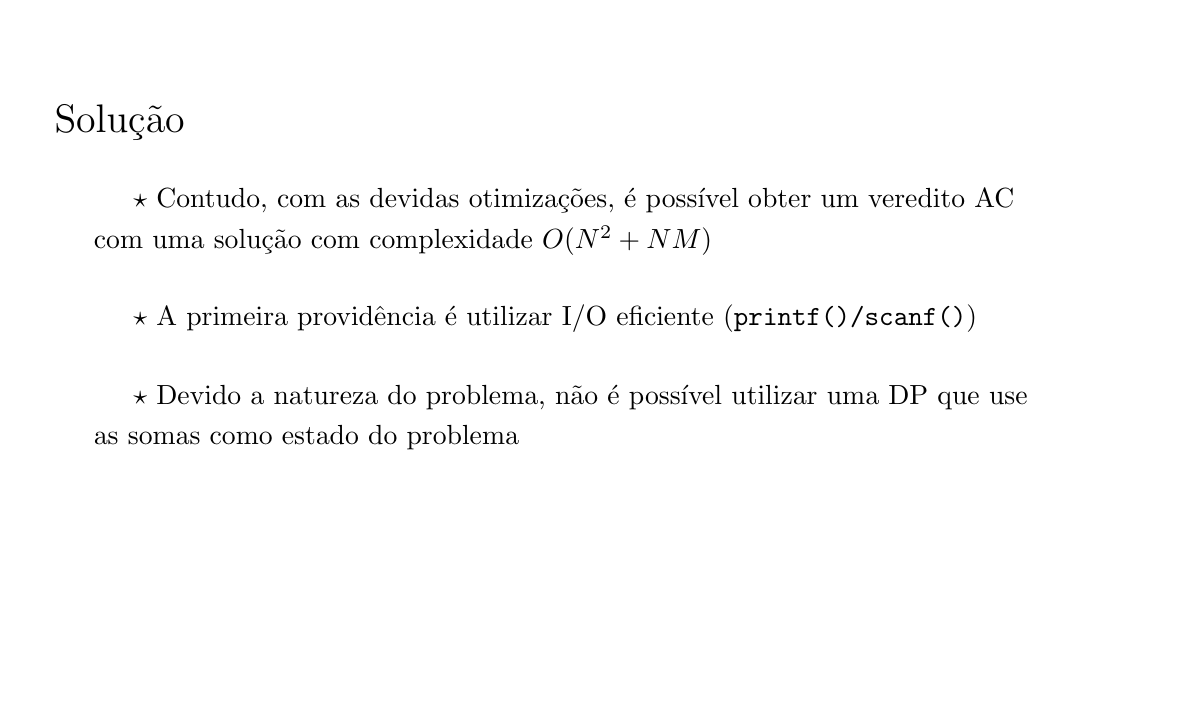
\begin{tikzpicture}
\node[draw,opacity=0] at (0, 0) {x};
\node[draw,opacity=0] at (14, 8) {x};

	\node[anchor=west] (title) at (0.0, 7.0) { \Large \bbbold{Solução} };

	\node[anchor=west] (a) at (1.0, 6.0) { $\star$ \bbtext{Contudo, com as devidas otimizações, é possível obter um veredito AC} };

	\node[anchor=west] (a1) at (0.5, 5.5) { \bbtext{com uma solução com complexidade $O(N^2 + NM)$} };


	\node[anchor=west] (b) at (1.0, 4.5) { $\star$ \bbtext{A primeira providência é utilizar I/O eficiente (\texttt{printf()/scanf()})} };


	\node[anchor=west] (c) at (1.0, 3.5) { $\star$ \bbtext{Devido a natureza do problema, não é possível utilizar uma DP que use} };

	\node[anchor=west] (c1) at (0.5, 3.0) { \bbtext{as somas como estado do problema} };

\end{tikzpicture}
\end{frame}
\begin{frame}[plain,t]
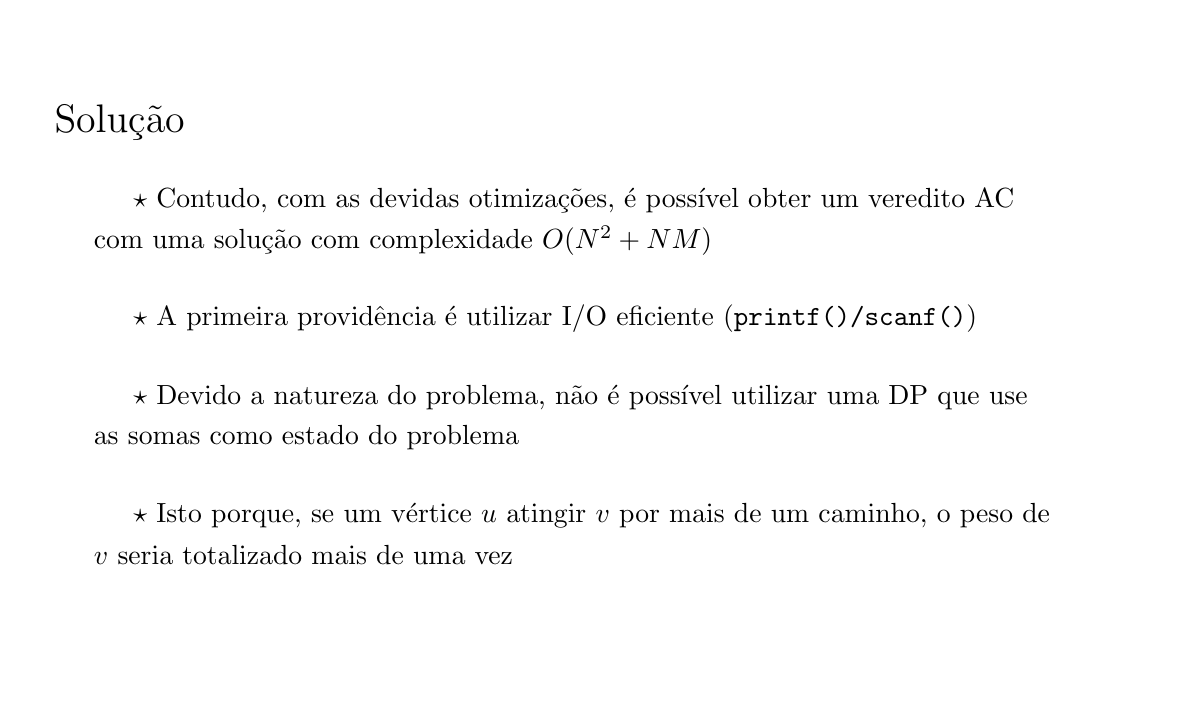
\begin{tikzpicture}
\node[draw,opacity=0] at (0, 0) {x};
\node[draw,opacity=0] at (14, 8) {x};

	\node[anchor=west] (title) at (0.0, 7.0) { \Large \bbbold{Solução} };

	\node[anchor=west] (a) at (1.0, 6.0) { $\star$ \bbtext{Contudo, com as devidas otimizações, é possível obter um veredito AC} };

	\node[anchor=west] (a1) at (0.5, 5.5) { \bbtext{com uma solução com complexidade $O(N^2 + NM)$} };


	\node[anchor=west] (b) at (1.0, 4.5) { $\star$ \bbtext{A primeira providência é utilizar I/O eficiente (\texttt{printf()/scanf()})} };


	\node[anchor=west] (c) at (1.0, 3.5) { $\star$ \bbtext{Devido a natureza do problema, não é possível utilizar uma DP que use} };

	\node[anchor=west] (c1) at (0.5, 3.0) { \bbtext{as somas como estado do problema} };


	\node[anchor=west] (d) at (1.0, 2.0) { $\star$ \bbtext{Isto porque, se um vértice $u$ atingir $v$ por mais de um caminho, o peso de} };

	\node[anchor=west] (d1) at (0.5, 1.5) { \bbtext{$v$ seria totalizado mais de uma vez} };

\end{tikzpicture}
\end{frame}
\begin{frame}[plain,t]
\begin{tikzpicture}
\node[draw,opacity=0] at (0, 0) {x};
\node[draw,opacity=0] at (14, 8) {x};

	\node[anchor=west] (title) at (0.0, 7.0) { \Large \bbbold{Solução} };

	\node[anchor=west] (a) at (1.0, 6.0) { $\star$ \bbtext{Seja $R[u]$ o conjunto do vértices alcancáveis a partir de $u$} };

\end{tikzpicture}
\end{frame}
\begin{frame}[plain,t]
\begin{tikzpicture}
\node[draw,opacity=0] at (0, 0) {x};
\node[draw,opacity=0] at (14, 8) {x};

	\node[anchor=west] (title) at (0.0, 7.0) { \Large \bbbold{Solução} };

	\node[anchor=west] (a) at (1.0, 6.0) { $\star$ \bbtext{Seja $R[u]$ o conjunto do vértices alcancáveis a partir de $u$} };


	\node[anchor=west] (b) at (1.0, 5.0) { $\star$ \bbtext{Se o grau de saída de $u$ é igual a zero, então $R[u] = \{\ u\ \}$} };

\end{tikzpicture}
\end{frame}
\begin{frame}[plain,t]
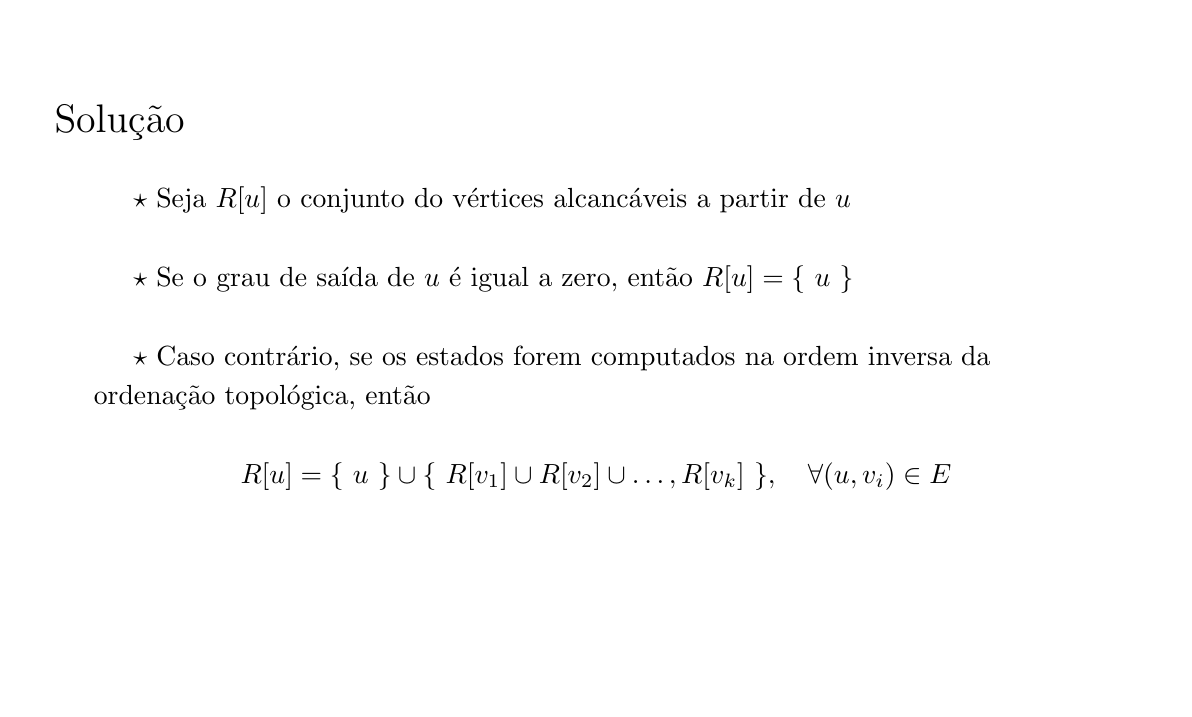
\begin{tikzpicture}
\node[draw,opacity=0] at (0, 0) {x};
\node[draw,opacity=0] at (14, 8) {x};

	\node[anchor=west] (title) at (0.0, 7.0) { \Large \bbbold{Solução} };

	\node[anchor=west] (a) at (1.0, 6.0) { $\star$ \bbtext{Seja $R[u]$ o conjunto do vértices alcancáveis a partir de $u$} };


	\node[anchor=west] (b) at (1.0, 5.0) { $\star$ \bbtext{Se o grau de saída de $u$ é igual a zero, então $R[u] = \{\ u\ \}$} };


	\node[anchor=west] (c) at (1.0, 4.0) { $\star$ \bbtext{Caso contrário, se os estados forem computados na ordem inversa da} };

	\node[anchor=west] (c1) at (0.5, 3.5) { \bbtext{ordenação topológica, então} };

	\node[] (c2) at (7.0, 2.5) { $\displaystyle R[u] = \{\ u\ \} \cup \{\ R[v_1]\cup R[v_2]\cup \ldots, R[v_k]\ \}, \ \ \ \forall (u, v_i)\in E$ };

\end{tikzpicture}
\end{frame}
\begin{frame}[plain,t]
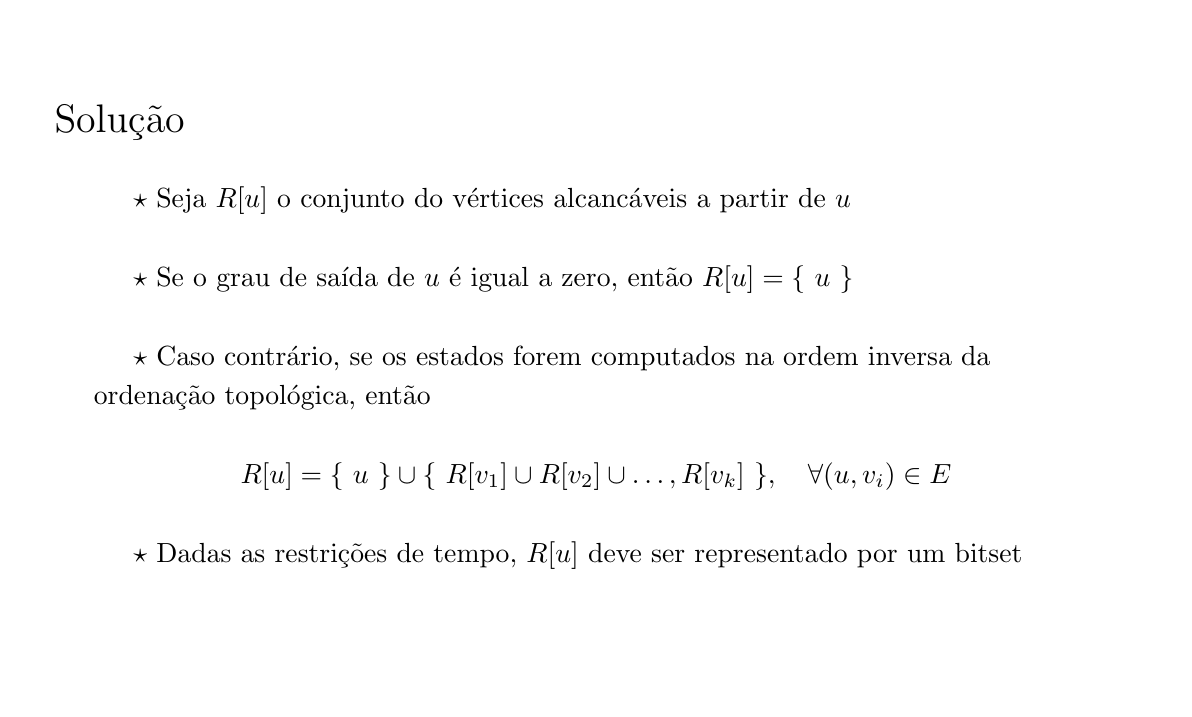
\begin{tikzpicture}
\node[draw,opacity=0] at (0, 0) {x};
\node[draw,opacity=0] at (14, 8) {x};

	\node[anchor=west] (title) at (0.0, 7.0) { \Large \bbbold{Solução} };

	\node[anchor=west] (a) at (1.0, 6.0) { $\star$ \bbtext{Seja $R[u]$ o conjunto do vértices alcancáveis a partir de $u$} };


	\node[anchor=west] (b) at (1.0, 5.0) { $\star$ \bbtext{Se o grau de saída de $u$ é igual a zero, então $R[u] = \{\ u\ \}$} };


	\node[anchor=west] (c) at (1.0, 4.0) { $\star$ \bbtext{Caso contrário, se os estados forem computados na ordem inversa da} };

	\node[anchor=west] (c1) at (0.5, 3.5) { \bbtext{ordenação topológica, então} };

	\node[] (c2) at (7.0, 2.5) { $\displaystyle R[u] = \{\ u\ \} \cup \{\ R[v_1]\cup R[v_2]\cup \ldots, R[v_k]\ \}, \ \ \ \forall (u, v_i)\in E$ };


	\node[anchor=west] (d) at (1.0, 1.5) { $\star$ \bbtext{Dadas as restrições de tempo, $R[u]$ deve ser representado por um \bbenglish{bitset}} };

\end{tikzpicture}
\end{frame}
\begin{frame}[plain,t]
\begin{tikzpicture}
\node[draw,opacity=0] at (0, 0) {x};
\node[draw,opacity=0] at (14, 8) {x};

	\node[anchor=west] (title) at (0.0, 7.0) { \Large \bbbold{Solução} };

	\node[anchor=west] (a) at (1.0, 6.0) { $\star$ \bbtext{Além disso, a implementação deste \bbenglish{bitset} deve ser customizada} };

\end{tikzpicture}
\end{frame}
\begin{frame}[plain,t]
\begin{tikzpicture}
\node[draw,opacity=0] at (0, 0) {x};
\node[draw,opacity=0] at (14, 8) {x};

	\node[anchor=west] (title) at (0.0, 7.0) { \Large \bbbold{Solução} };

	\node[anchor=west] (a) at (1.0, 6.0) { $\star$ \bbtext{Além disso, a implementação deste \bbenglish{bitset} deve ser customizada} };


	\node[anchor=west] (b) at (1.0, 5.0) { $\star$ \bbtext{Se os elementos são representados em $R[u]$ por seus índices na ordenação} };

	\node[anchor=west] (b1) at (0.5, 4.5) { \bbtext{topológica, a união pode ser feita de forma mais eficiente} };


\end{tikzpicture}
\end{frame}
\begin{frame}[plain,t]
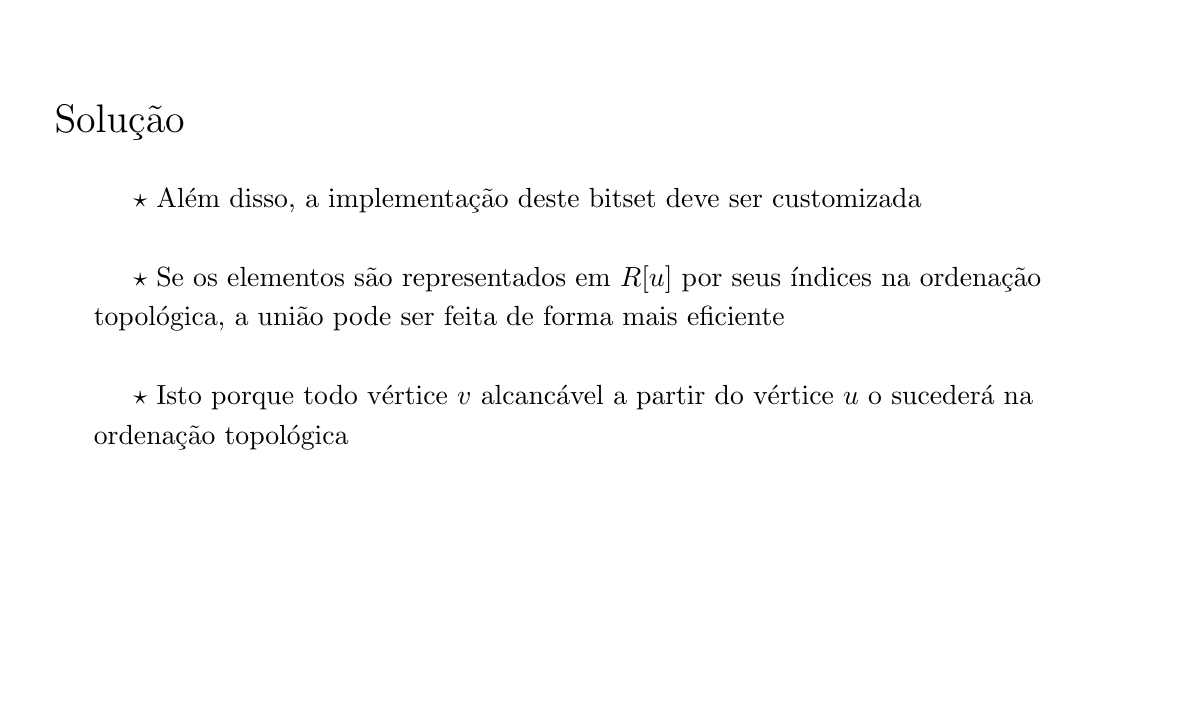
\begin{tikzpicture}
\node[draw,opacity=0] at (0, 0) {x};
\node[draw,opacity=0] at (14, 8) {x};

	\node[anchor=west] (title) at (0.0, 7.0) { \Large \bbbold{Solução} };

	\node[anchor=west] (a) at (1.0, 6.0) { $\star$ \bbtext{Além disso, a implementação deste \bbenglish{bitset} deve ser customizada} };


	\node[anchor=west] (b) at (1.0, 5.0) { $\star$ \bbtext{Se os elementos são representados em $R[u]$ por seus índices na ordenação} };

	\node[anchor=west] (b1) at (0.5, 4.5) { \bbtext{topológica, a união pode ser feita de forma mais eficiente} };



	\node[anchor=west] (c) at (1.0, 3.5) { $\star$ \bbtext{Isto porque todo vértice $v$ alcancável a partir do vértice $u$ o sucederá na} };

	\node[anchor=west] (c1) at (0.5, 3.0) { \bbtext{ordenação topológica} };

\end{tikzpicture}
\end{frame}
\begin{frame}[plain,t]
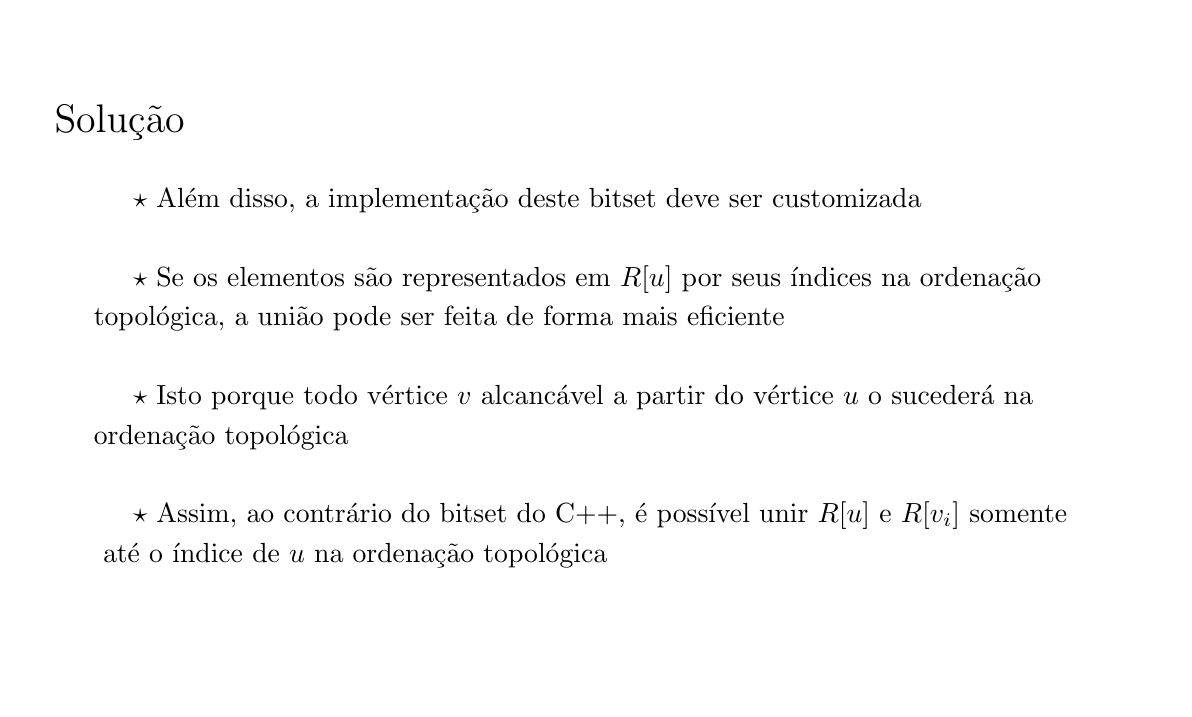
\begin{tikzpicture}
\node[draw,opacity=0] at (0, 0) {x};
\node[draw,opacity=0] at (14, 8) {x};

	\node[anchor=west] (title) at (0.0, 7.0) { \Large \bbbold{Solução} };

	\node[anchor=west] (a) at (1.0, 6.0) { $\star$ \bbtext{Além disso, a implementação deste \bbenglish{bitset} deve ser customizada} };


	\node[anchor=west] (b) at (1.0, 5.0) { $\star$ \bbtext{Se os elementos são representados em $R[u]$ por seus índices na ordenação} };

	\node[anchor=west] (b1) at (0.5, 4.5) { \bbtext{topológica, a união pode ser feita de forma mais eficiente} };



	\node[anchor=west] (c) at (1.0, 3.5) { $\star$ \bbtext{Isto porque todo vértice $v$ alcancável a partir do vértice $u$ o sucederá na} };

	\node[anchor=west] (c1) at (0.5, 3.0) { \bbtext{ordenação topológica} };


	\node[anchor=west] (d) at (1.0, 2.0) { $\star$ \bbtext{Assim, ao contrário do \bbenglish{bitset} do C++, é possível unir $R[u]$ e $R[v_i]$ somente} };

	\node[anchor=west] (d1) at (0.5, 1.5) { \bbtext{ até o índice de $u$ na ordenação topológica} };


\end{tikzpicture}
\end{frame}
\begin{frame}[plain,t]

\inputsnippet{cpp}{46}{65}{codes/DAGCNT2.cpp}

\end{frame}
\begin{frame}[plain,t]

\inputsnippet{cpp}{41}{44}{codes/DAGCNT2.cpp}


\end{frame}
\end{document}
